%!TeX root=MemoriaTFG.tex

\chapter{Implementation}\label{chap:implementation}

\section{Application composition}\label{sec:implementation-composition}

The architectural chapter introduced the decision to use manual composition. In the implementation, this responsibility belongs to the static \texttt{AppComposition} class. Its initialization method first creates the application directories, then the JSON repositories, HTTP catalogues, installers, Windows process executor, SharpOpenNat mapper and image transformer. It uses these adapters to construct the intermediate managers, followed by the input services. Finally, small factory methods return fully initialized view models to the pages.

This is one of the less elegant parts of the code because the construction section is sizeable and the complete graph has a static lifetime. For a single local application instance, I found that trade-off acceptable. The benefit during development was practical: when a service required a new dependency, the complete construction path was visible in one file. If the application grows, smaller composition modules could make tests easier to set up without changing the architectural boundaries.

The following shortened excerpt from \texttt{AppComposition} illustrates why the selected approach remains easy to follow. Each service is constructed from previously created ports, and its dependencies can be identified without consulting registration rules or framework conventions.

\begin{footnotesize}
\begin{verbatim}
serverPathResolver = new ServerPathResolver(
    appDirectory, serversDirectory, tmpDirectory);
propertiesManagerService = new PropertiesManagerService(
    serverPathResolver, serverPropertiesRepository);
eulaManagerService = new EulaManagerService(
    serverPathResolver, serverEulaRepository);
versionManagerService = new VersionManagerService(
    serverPathResolver, minecraftVersionRepository);
\end{verbatim}
\end{footnotesize}

The excerpt also shows the dependency direction in practice. \texttt{PropertiesManagerService} receives an \texttt{IServerPropertiesRepository}; it never creates a JSON or text repository internally. The same rule is followed by the EULA and version managers. As a result, the implementation can replace one adapter without changing the manager that uses its contract.

At startup, four logical storage locations are derived from MAUI's application-data directory: the application root, \texttt{Servers}, \texttt{Java} and \texttt{tmp}. Provider adapters use the temporary location for downloaded packages, while repositories and the path resolver use the persistent locations. The program does not assume that its installation folder is writable.

\section{Server persistence and file management}

\subsection{JSON repositories}

\texttt{JsonServerRepository}, \texttt{JsonJavaRepository} and \texttt{JsonApplicationConfigurationRepository} implement the persistent stores. Their interfaces make save, retrieval and removal explicit while shielding callers from filenames and serializer settings. A server's identifier is stable and is used both to distinguish records and to derive its managed directory.

Application configuration includes the default Java selection and the CurseForge API token. The configuration service trims the token and propagates it to CurseForge supplier instances. Keeping this operation in a service ensures that a token loaded at startup and a token changed through the settings view have the same effect.

JSON was not used for Minecraft's own settings. The server expects \texttt{server.properties} and \texttt{eula.txt}, so specialized repositories write those native formats. This distinction avoids treating every file as an application database record. Wave metadata describes the managed aggregate; Minecraft files remain in the form consumed by Minecraft.

\subsection{Paths and cleanup}

\texttt{ServerPathResolver} supplies paths for the root, vanilla JAR, loader JAR, properties, EULA and mods. Services request paths instead of reconstructing names. Creation ensures required directories exist, while deletion removes the complete server root only for the selected managed instance.

Temporary installer files are removed after successful use. Mod downloads are also guarded by cleanup: if a supplier throws during a download, artifacts known for that mod are removed when possible and the operation is reported as failed. Cleanup exceptions are logged separately so they do not hide the original failure.

\section{Minecraft catalogue and installation}

\texttt{ApiMinecraftVersionRepository} reads Mojang's global version manifest. Each entry is mapped to a domain item that identifies releases, snapshots and pre-releases and retains the URL for detailed metadata. When a user selects a version, the repository follows that URL to obtain the server download and Java information, then streams the JAR to the destination chosen by the path resolver.

The catalogue service filters snapshots unless the query enables them. This preserves the full provider catalogue without burdening the usual creation workflow with unstable releases. Property definitions are held by an in-memory repository because they are part of the interface model rather than remote changing data. Their keys correspond to Minecraft's \texttt{server.properties} format, and their types determine which form component is created.

\texttt{VersionManagerService} distinguishes a catalogue choice from the already installed selection. When the versions differ, it retrieves details and replaces the managed vanilla artifact. This service is called by server creation and by editing, allowing both workflows to use the same installation behavior.

\section{Java runtime management}

\subsection{Supplier adapters}

Java support has two supplier adapters. The Adoptium adapter queries available feature releases for the device operating system and architecture, maps returned binary metadata and downloads a compressed package. The Mojang adapter obtains its runtime manifest and downloads the set of files described by the selected release.

These delivery formats are intentionally different in the implementation. \texttt{CompressedJavaPackage} is handled by \texttt{CompressedJavaInstaller}, which extracts ZIP or TAR-based archives, locates the Java executable and places the installation beneath the managed Java directory. \texttt{ManifestJavaPackage} is handled by \texttt{ManifestJavaInstaller}, which reconstructs Mojang's file tree from manifest entries and assigns executable information. The abandoned MSI path is not part of the active project. Adoptium is installed only from compressed packages, avoiding system-wide installer behavior and administrative side effects.

\subsection{Selection and removal}

The Java settings view obtains device information from \texttt{WindowsDeviceInformationRepository} and uses it to restrict supplier queries. Installed runtimes are read from the Java repository. After installation, the normalized domain object records supplier, version, artifact type, executable and removal location.

Before uninstalling a runtime, the Java manager checks the saved servers. Removal is refused if any server refers to that installation, preventing a configuration from retaining a dead executable path. A different runtime can first be assigned through the server editor. This rule is implemented in the use-case service rather than only in the interface, so it also protects future callers.

\begin{figure}[htbp]
  \centering
  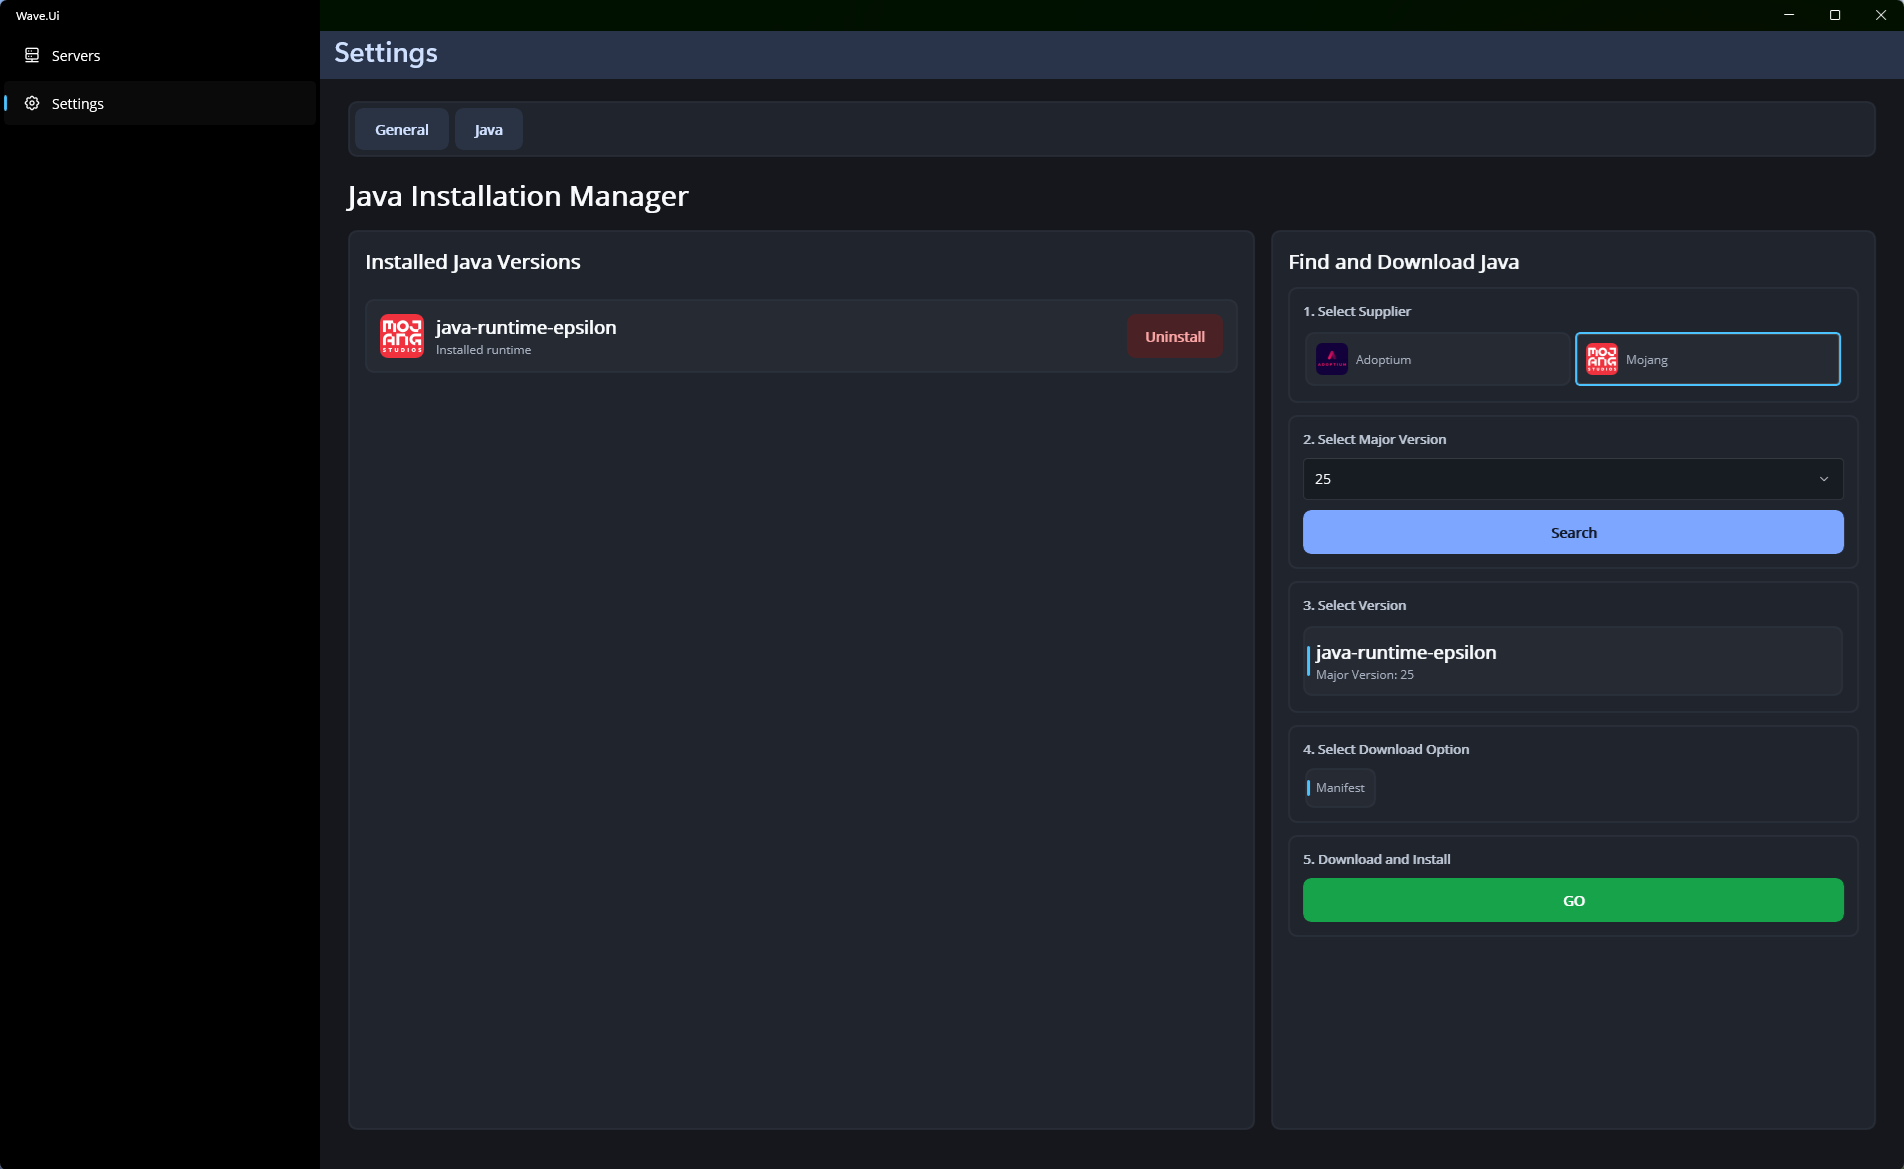
\includegraphics[width=\textwidth,height=0.72\textheight,keepaspectratio]{JavaSettings.png}
  \caption{Java catalogue, package and installation screens.}
  \label{fig:java-ui}
\end{figure}

\section{Forge and Fabric integration}

Forge publishes version bundles through Maven metadata. \texttt{ApiForgeVersionCatalog} downloads and deserializes the XML document, maps each combined Minecraft and Forge version, filters it for the requested Minecraft release and reverses the result so recent releases appear first. The selected installer JAR is downloaded from the corresponding Maven path.

Fabric supplies loader and installer information through JSON endpoints. Its adapter combines the selected loader with a current installer package. Both adapters implement \texttt{IModloaderVersionCatalog}; callers select them by \texttt{ModloaderType} and do not handle XML or Fabric DTOs.

Installation invokes the downloaded JAR with a managed Java executable in server-install mode. When the installer completes successfully, the resulting launcher JAR is located and moved to the normalized loader path. The stored \texttt{ModloaderInstallation} retains type, Minecraft version and loader version. Temporary installer material is then cleared.

Loader migration begins only when the server already has a loader. The catalogue is queried using the new Minecraft version. If there is no corresponding release, loader state is removed. Otherwise the old loader is removed, the first compatible catalogue result is installed and mod migration can continue against the new combination.

\section{Mod provider integration}

\subsection{Common supplier contract}

\texttt{IModSupplierIntegration} covers search, project details, compatible versions, download and token configuration. A supplier declares which \texttt{ModSupplierType} it handles. \texttt{ModCatalogService} selects the appropriate adapter, checks whether its configuration permits use and returns provider-independent domain data to the interface.

Search is paginated. The UI query includes Minecraft version and loader, which adapters translate into the filters required by their provider. Results expose a project name, summary, icon and provider identifier. Selecting a project triggers separate detail and version requests so the initial results remain compact.

\subsection{Modrinth}

The Modrinth adapter uses its project search and version operations without requiring a user API token. DTO mappers translate project type, authors, descriptions, files and dependency relations. File downloads are streamed into the server's mods directory. Markdown descriptions are converted for presentation in the mod popup.

\subsection{CurseForge}

CurseForge requests include an API token stored through the settings page. Operations fail with a clear configuration exception when the token is empty. The adapter maps CurseForge project and file identifiers into the same domain model used by Modrinth, while retaining supplier identity so later detail and download calls return to the correct platform.

The provider uses dependency classifications that do not map perfectly to the subset required by the application. Required and incompatible relations participate in automatic resolution. Unsupported relation types remain an adapter concern and are not silently treated as required dependencies.

\begin{figure}[htbp]
  \centering
  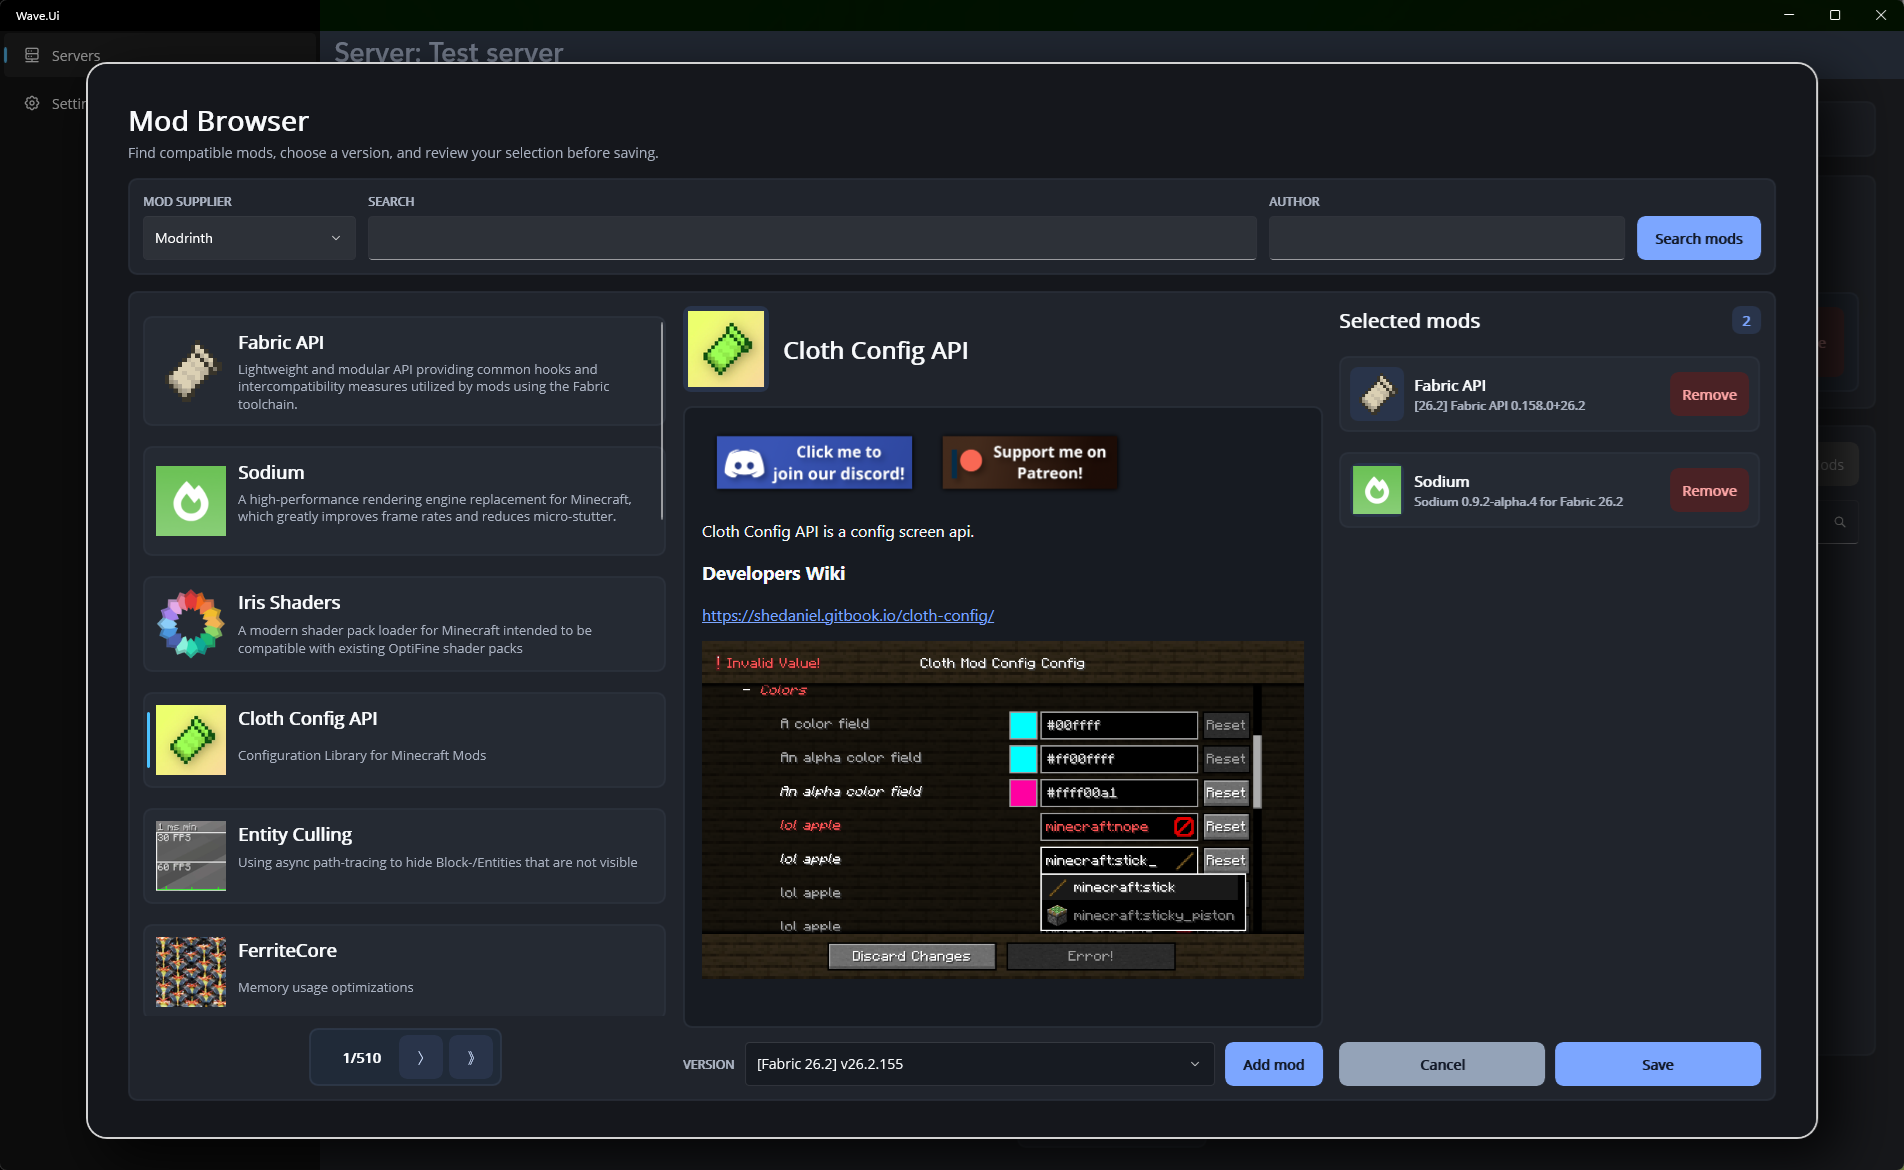
\includegraphics[width=\textwidth,height=0.72\textheight,keepaspectratio]{ModBrowser.png}
  \caption{Mod search, details and selected-mod views.}
  \label{fig:mods-ui}
\end{figure}

\section{Dependency installation and migration}

\texttt{ModManagerService} compares requested and installed mods using the pair of project and version identifiers. Added items pass through recursive dependency resolution before download. Removed items have each known artifact deleted and are removed from server metadata.

Required dependency resolution receives the candidate, current server state, explicitly known selections, an accumulating dependency list and a visiting set. It first tests incompatibilities against installed and planned items. It then follows every required relation that is not already satisfied. If the dependency was explicitly selected, that exact selection can be reused. Otherwise the supplier is queried for a compatible version and its project information. Recursion processes the dependency's own requirements before adding it to the ordered download list.

The visiting set handles circular declarations. Encountering the same project on the current recursive path returns success rather than descending again. A project is added only once because installed and planned lists are checked at each step. These two guards protect against both cycles and repeated dependencies shared by several selected mods.

The central guard and recursive call in \texttt{ResolveDependenciesAsync} make this behavior explicit. The visiting set terminates a cycle, while any non-successful result from a nested dependency is propagated to the original installation request.

\begin{footnotesize}
\begin{verbatim}
if (!visiting.Add(mod.ModId))
    return DependencyResolution.Success;

var result = await ResolveDependenciesAsync(
    dependencyMod,
    server,
    knownMods,
    dependencyMods,
    visiting);
if (result != DependencyResolution.Success)
    return result;
\end{verbatim}
\end{footnotesize}

Downloads occur after resolution for each candidate. Automatically obtained dependencies are installed before the requesting mod. The result returns automatically required items as well as failures and incompatibilities. This lets the popup explain why the final set differs from the user's direct selection.

Migration uses the new Minecraft version and loader as its compatibility query. Each outdated mod artifact is uninstalled and the supplier is asked for alternatives. No available release means the mod is recorded as deleted. A replacement is processed through the same dependency routine used for ordinary additions. The interface can therefore present one consolidated migration result rather than leaving obsolete files in the directory.

\begin{figure}[htbp]
  \centering
  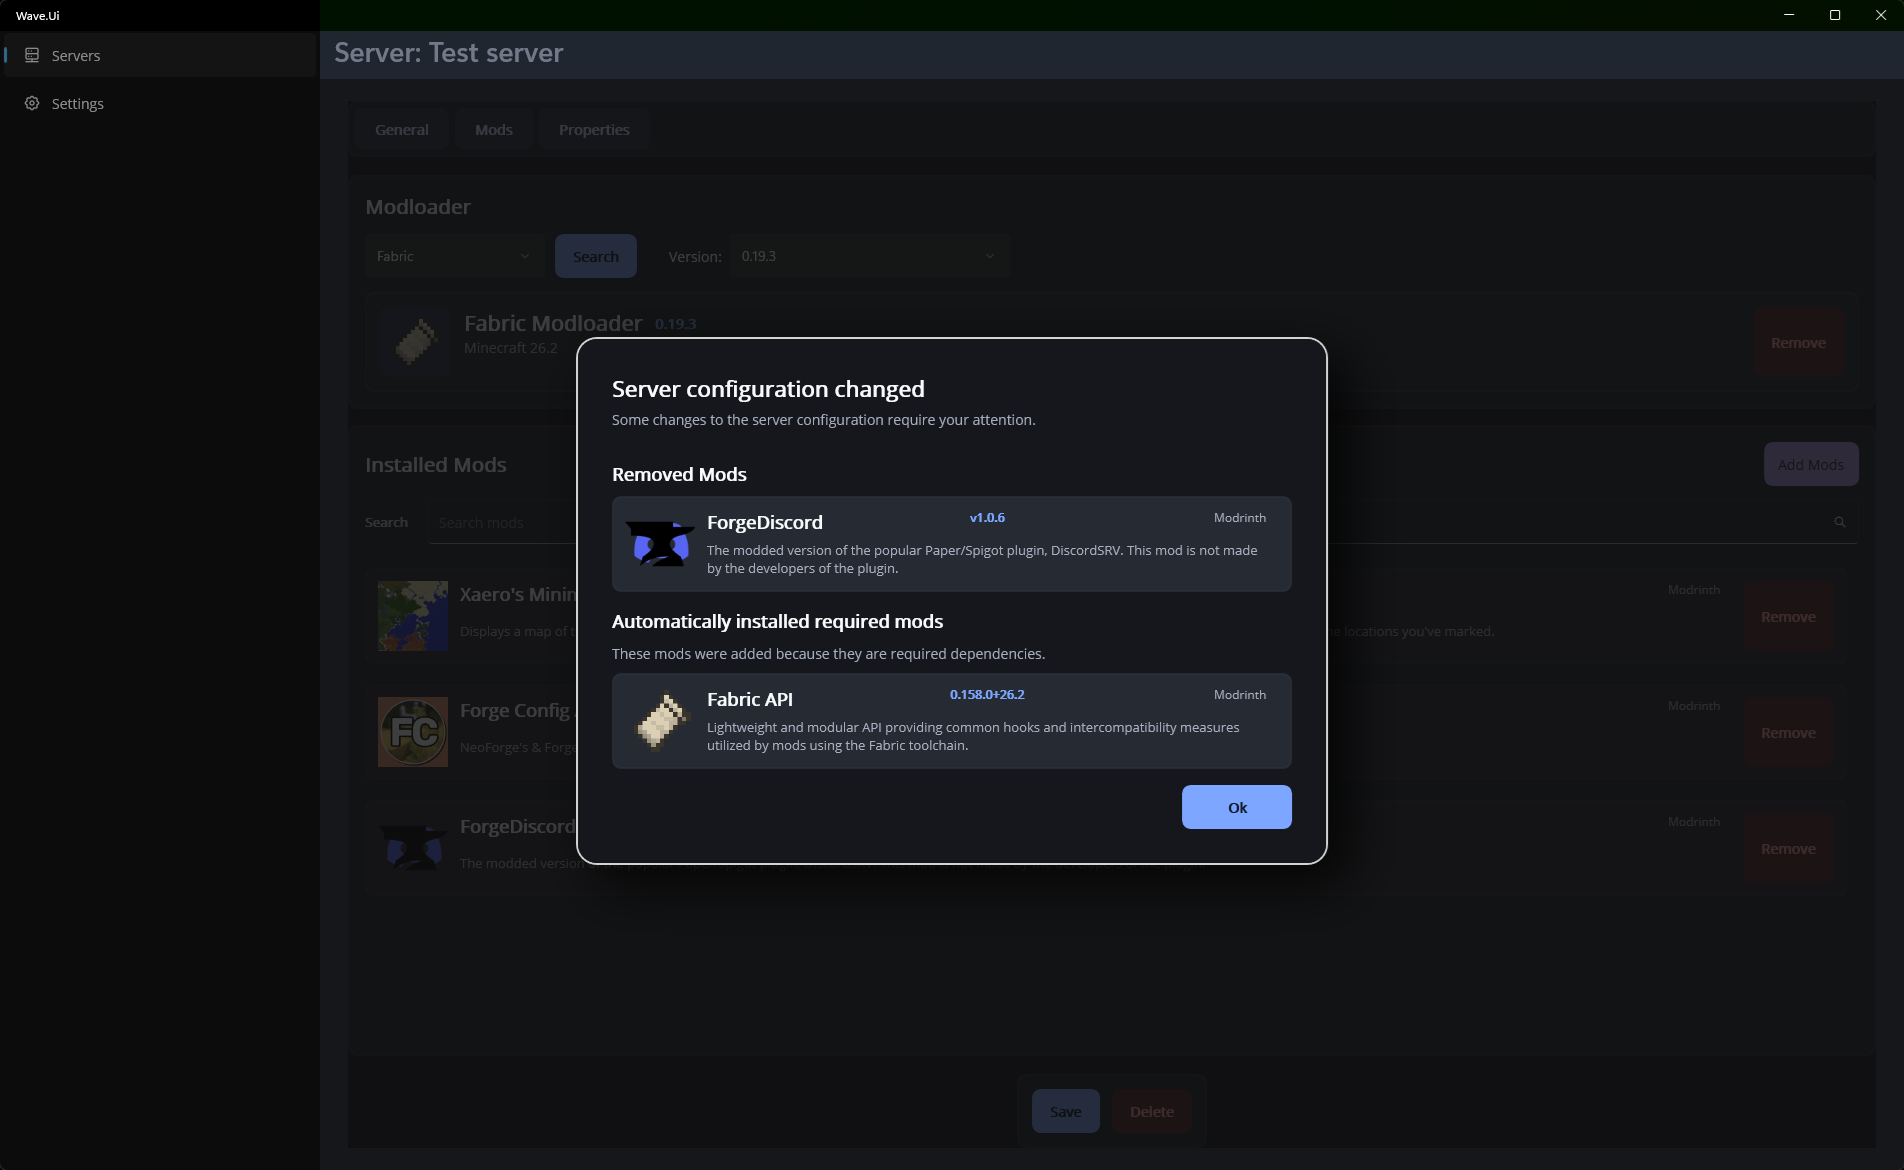
\includegraphics[width=\textwidth,height=0.72\textheight,keepaspectratio]{ChangeSummary.png}
  \caption{Change summary produced during a server-version migration.}
  \label{fig:migration-ui}
\end{figure}

\section{Server creation and update orchestration}

\texttt{ServerManagerService} owns workflows that span several specialized managers. Creation initializes the server from the submitted query, creates the root, installs the Minecraft version, writes properties and EULA state, installs an optional loader, adds selected mods, transforms the icon and saves the final aggregate.

The implementation keeps this order visible instead of hiding it in a generic pipeline. The following shortened fragment from \texttt{CreateServerAsync} shows the main sequence. Each call delegates one concern, while the service remains responsible for coordinating the complete use case.

\begin{footnotesize}
\begin{verbatim}
serverPathResolver.CreateServerRootDirectory(server);
server = await versionManagerService.SetVersionAsync(server, query);

serverPathResolver.CreateServerPropertiesFile(server);
await propertiesManagerService.SetPropertiesAsync(server);

serverPathResolver.CreateEulaFile(server);
await eulaManagerService.SetEulaAsync(server, query);

await modloaderManagerService.AddModloaderAsync(server, query);
await modManagerService.SetModsAsync(server, query);
await serverRepository.SaveServerAsync(server);
\end{verbatim}
\end{footnotesize}

This order matters. The version manager needs an existing root in which to place the server JAR, and the loader and mod managers need a concrete Minecraft installation against which compatibility can be checked. Persistence comes last so that a newly created record does not claim success before the main artifacts have been installed.

Update is more involved. It loads the existing aggregate, remembers the original Minecraft version and loader, and applies the submitted values. Version migration comes before loader and mod migration because their valid choices depend on Minecraft. If the loader type changes, the old loader is removed before the new one is installed. The method then either migrates the mods or applies an ordinary mod-set change. Failures, incompatibilities, deleted mods and automatically required dependencies are combined into \texttt{ServerChanges}. This object is returned only when there is something the user should be told about.

The service also supplies a preview of changes for the popup. A change object communicates version replacement and dependent modifications without making XAML calculate domain consequences. This division helped during UI development because the preview and final operation could evolve together in the application layer.

Deletion removes the server metadata and its managed directory. The UI prevents ordinary editing while an operation is in progress, but execution and management are separate services. A production-hardening step would add an application-level rule that makes deletion of a running server impossible even for a caller outside the current UI.

\section{Process execution and console}

\texttt{WindowsServerExecutor} creates a process using the selected Java executable. Its working directory is the server root, its arguments include configured execution flags and the appropriate server or mod-loader JAR, and shell execution is disabled. Standard streams are redirected and no additional console window is created.

The returned \texttt{ServerSession} exposes output and lifecycle information. Standard output and error are observed by \texttt{ExecutionViewModel}, which maintains the log shown in the execution page. Commands are written to the process input. Stopping requests Minecraft's normal stop command before session cleanup, allowing the game server to save world state.

Log distribution is implemented inside \texttt{ServerSession}. Two asynchronous pumps read the process's standard-output and standard-error streams line by line. Each produced line is written into a circular array at \texttt{bufferIndex modulo bufferSize}; the index then advances and a task-completion signal wakes consumers waiting for new output. Access to the array, index and completion state is protected by a lock, so both pumps can publish without corrupting their shared state. The current buffer contains ten lines, which bounds its memory use and retains the most recent output when producers advance faster than a consumer.

\texttt{GetOutputAsync} exposes this data as an \texttt{IAsyncEnumerable<string>}. Every invocation maintains its own \texttt{previousIndex}, copies the unread portion of the circular buffer while holding the lock, releases the lock before yielding the lines, and then waits on the current production signal. Consumers therefore do not remove entries from a shared queue. Several independent consumers can follow the same session concurrently, each progressing at its own rate. Cancellation stops only the corresponding enumeration, while completion of both stream pumps wakes all remaining consumers so their enumerations can finish normally.

The important detail is that no value is yielded while the lock is held. The method first copies the currently unread lines into a local queue, then returns them to the consumer. The central part of that operation is shown below.

\begin{footnotesize}
\begin{verbatim}
lock (bufferLock)
{
    currentIndex = bufferIndex;
    long unreadLines = currentIndex - previousIndex;
    long retainedLines = Math.Min(bufferSize, unreadLines);

    for (long i = currentIndex - retainedLines; i < currentIndex; i++)
        currentBuffer.Enqueue(buffer[i % bufferSize]);

    waitProduced = signal.Task;
    if (completed) shouldBreak = true;
}

foreach (string line in currentBuffer)
    yield return line;
\end{verbatim}
\end{footnotesize}

The names in this excerpt have been shortened slightly for readability, but the control flow matches \texttt{ServerSession}. Copying before yielding avoids holding a synchronization primitive across consumer code, which could otherwise delay both output pumps.

The UI is currently one such consumer, but the design allows other output processors to subscribe without changing process execution. A future persistence component could consume the same stream and write the server log to a text file for later consultation. Another component could inspect reported events and trigger configured actions, such as moderating a player when prohibited language is reported or restarting a server after Minecraft reports that a game tick is taking too long. These extensions should parse known message formats and apply explicit policies rather than embedding them in \texttt{ServerSession}, whose responsibility remains output distribution.

The circular buffer is a live distribution mechanism, not a durable log. A newly attached consumer receives at most the retained lines, and a consumer that falls more than ten lines behind can lose overwritten output. Reliable file logging would consequently require the persistence consumer to remain active and keep pace, or a later revision to introduce a larger buffer, backpressure or a dedicated durable logging channel.

\texttt{ServerExecutorService} maintains an in-memory dictionary from server identifiers to running-session records. A record also contains its port and mapping lease. The dictionary prevents duplicate starts and lets the servers page display current execution state. Because it is deliberately transient, restarting Wave Launcher begins with no claimed sessions.

\begin{figure}[htbp]
  \centering
  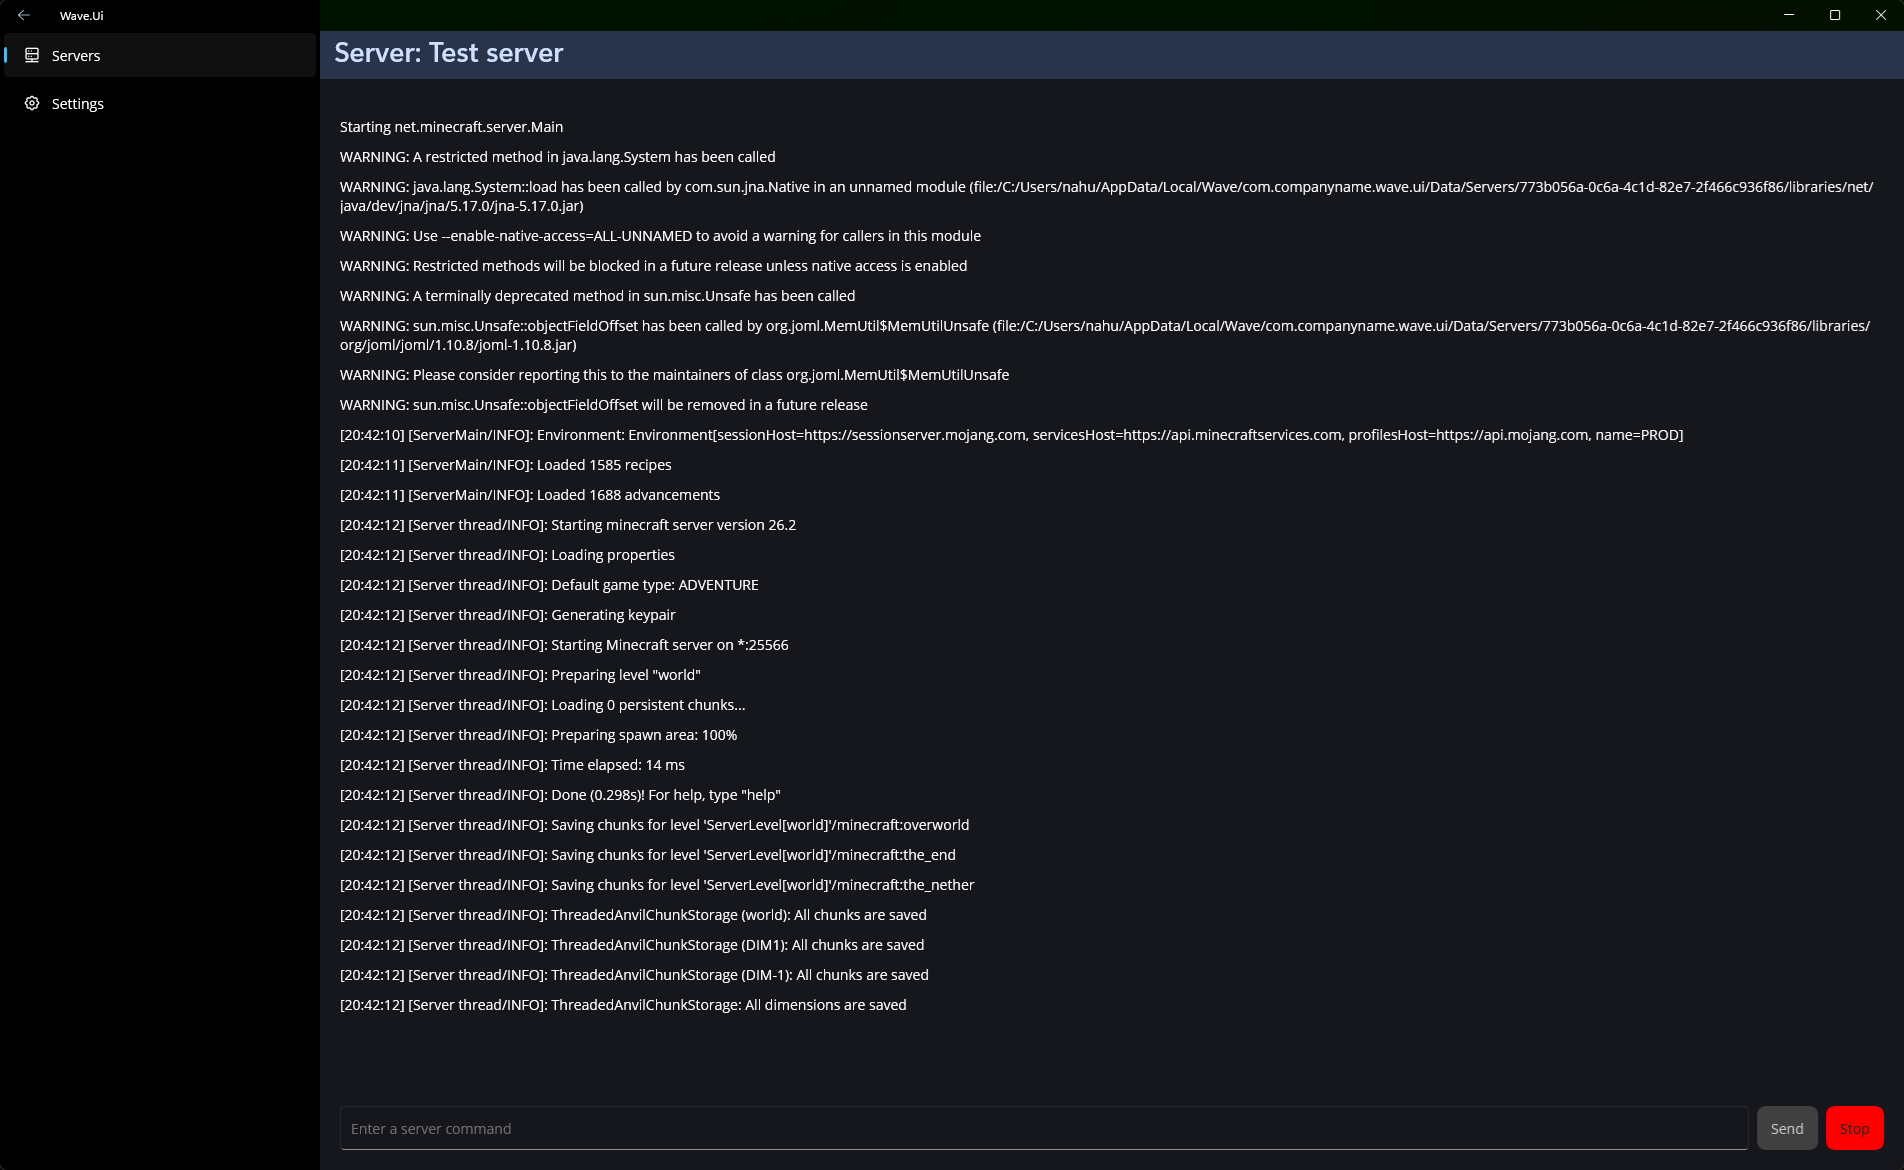
\includegraphics[width=\textwidth,height=0.72\textheight,keepaspectratio]{ServerExecutionPage.png}
  \caption{Execution page with redirected server output and command entry.}
  \label{fig:execution-ui}
\end{figure}

\section{Automatic port mapping}

The requested server port is read from the properties dictionary, with Minecraft's default used when the value is absent or invalid. The executor service checks its own running records for a conflict before making any network change. It then calls \texttt{IPortMapper.OpenAsync}.

\texttt{SharpOpenNatPortMapper} tries supported discovery protocols with a bounded timeout. For UPnP it can inspect a specific existing mapping. If an equivalent mapping already targets the local host and port, the adapter returns a lease without duplicating it. Otherwise it creates a TCP mapping whose public and private ports match. The returned \texttt{PortMappingLease} contains the cleanup action needed to remove a mapping created for the session.

If mapping fails, \texttt{ServerStartResult} reports the failure and process creation does not proceed. If process creation fails after mapping, the lease is disposed in the error path. Normal stop and observed process exit also dispose it. This sequence prevents a successful network side effect from being orphaned by a later local failure.

The lease itself contains only the mapped port and the operation required to release it. Its disposal guard is atomic, so cleanup can safely be requested by both explicit stopping and process-exit handling without removing the mapping twice.

\begin{footnotesize}
\begin{verbatim}
public async ValueTask DisposeAsync()
{
    if (Interlocked.Exchange(ref disposed, 1) != 0) return;
    await releaseAsync();
}
\end{verbatim}
\end{footnotesize}

Automatic mapping cannot guarantee external reachability. Some routers disable discovery, some networks place users behind carrier-grade \acs{NAT}, and host firewalls can still reject traffic. The implementation removes the need for manual router configuration when the local environment supports UPnP or NAT-PMP, while failure feedback remains necessary for unsupported networks.

\section{MAUI user interface}

\subsection{Shell and pages}

\texttt{AppShell} defines navigation among servers, execution and settings. Each content area uses a page, a view model and smaller views. The server editor, for example, composes general, property and mod views instead of placing the complete form in one XAML file. This mirrors the functional grouping used in the domain and keeps provider browsing separate from basic server identity.

Server cards show identifying and state information. The selected server is passed to the editor through its view model, where a query model collects changes. The same editor can represent a new or existing server, reducing divergence between creation and update validation.

\begin{figure}[htbp]
  \centering
  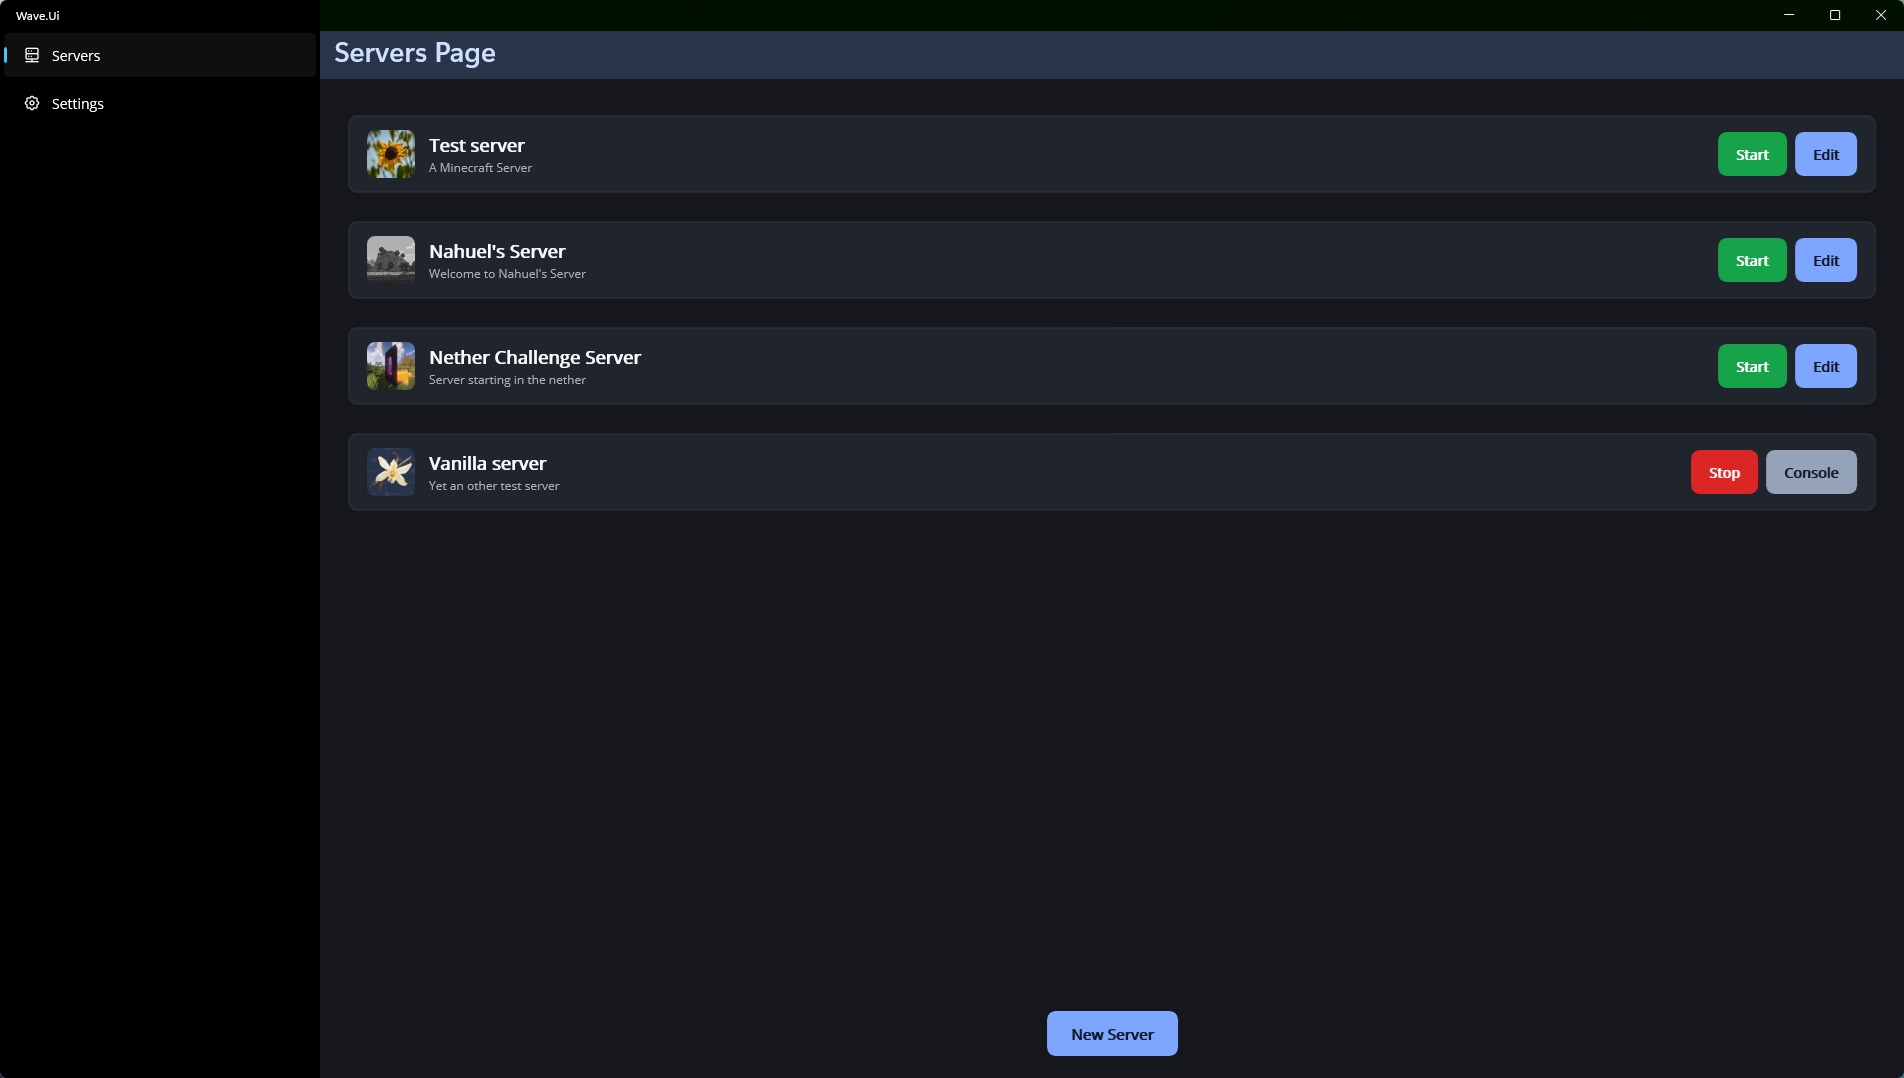
\includegraphics[width=\textwidth,height=0.72\textheight,keepaspectratio]{ServersPage.png}
  \caption{Server list page.}
  \label{fig:servers-page}
\end{figure}

\begin{figure}[htbp]
  \centering
  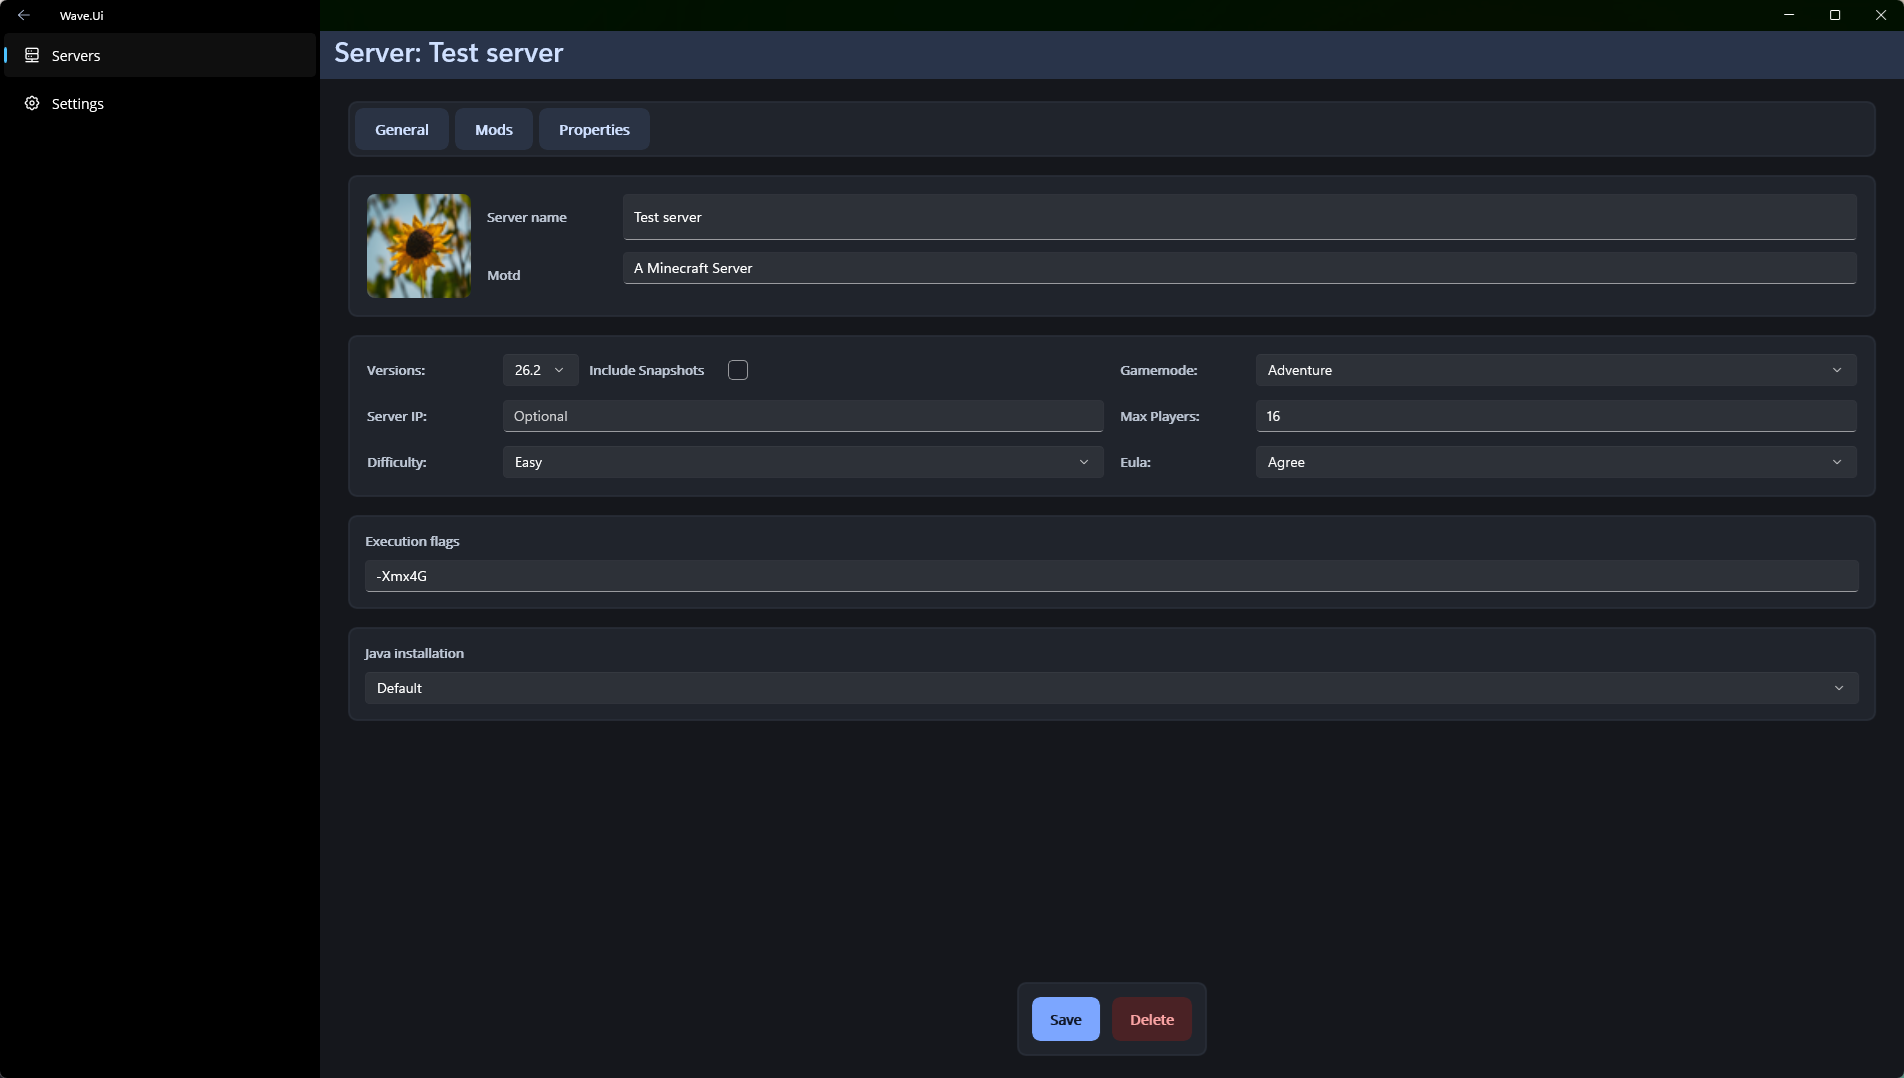
\includegraphics[width=\textwidth,height=0.72\textheight,keepaspectratio]{ServerConfigurationPage.png}
  \caption{General server-configuration page.}
  \label{fig:server-general-configuration}
\end{figure}

\begin{figure}[htbp]
  \centering
  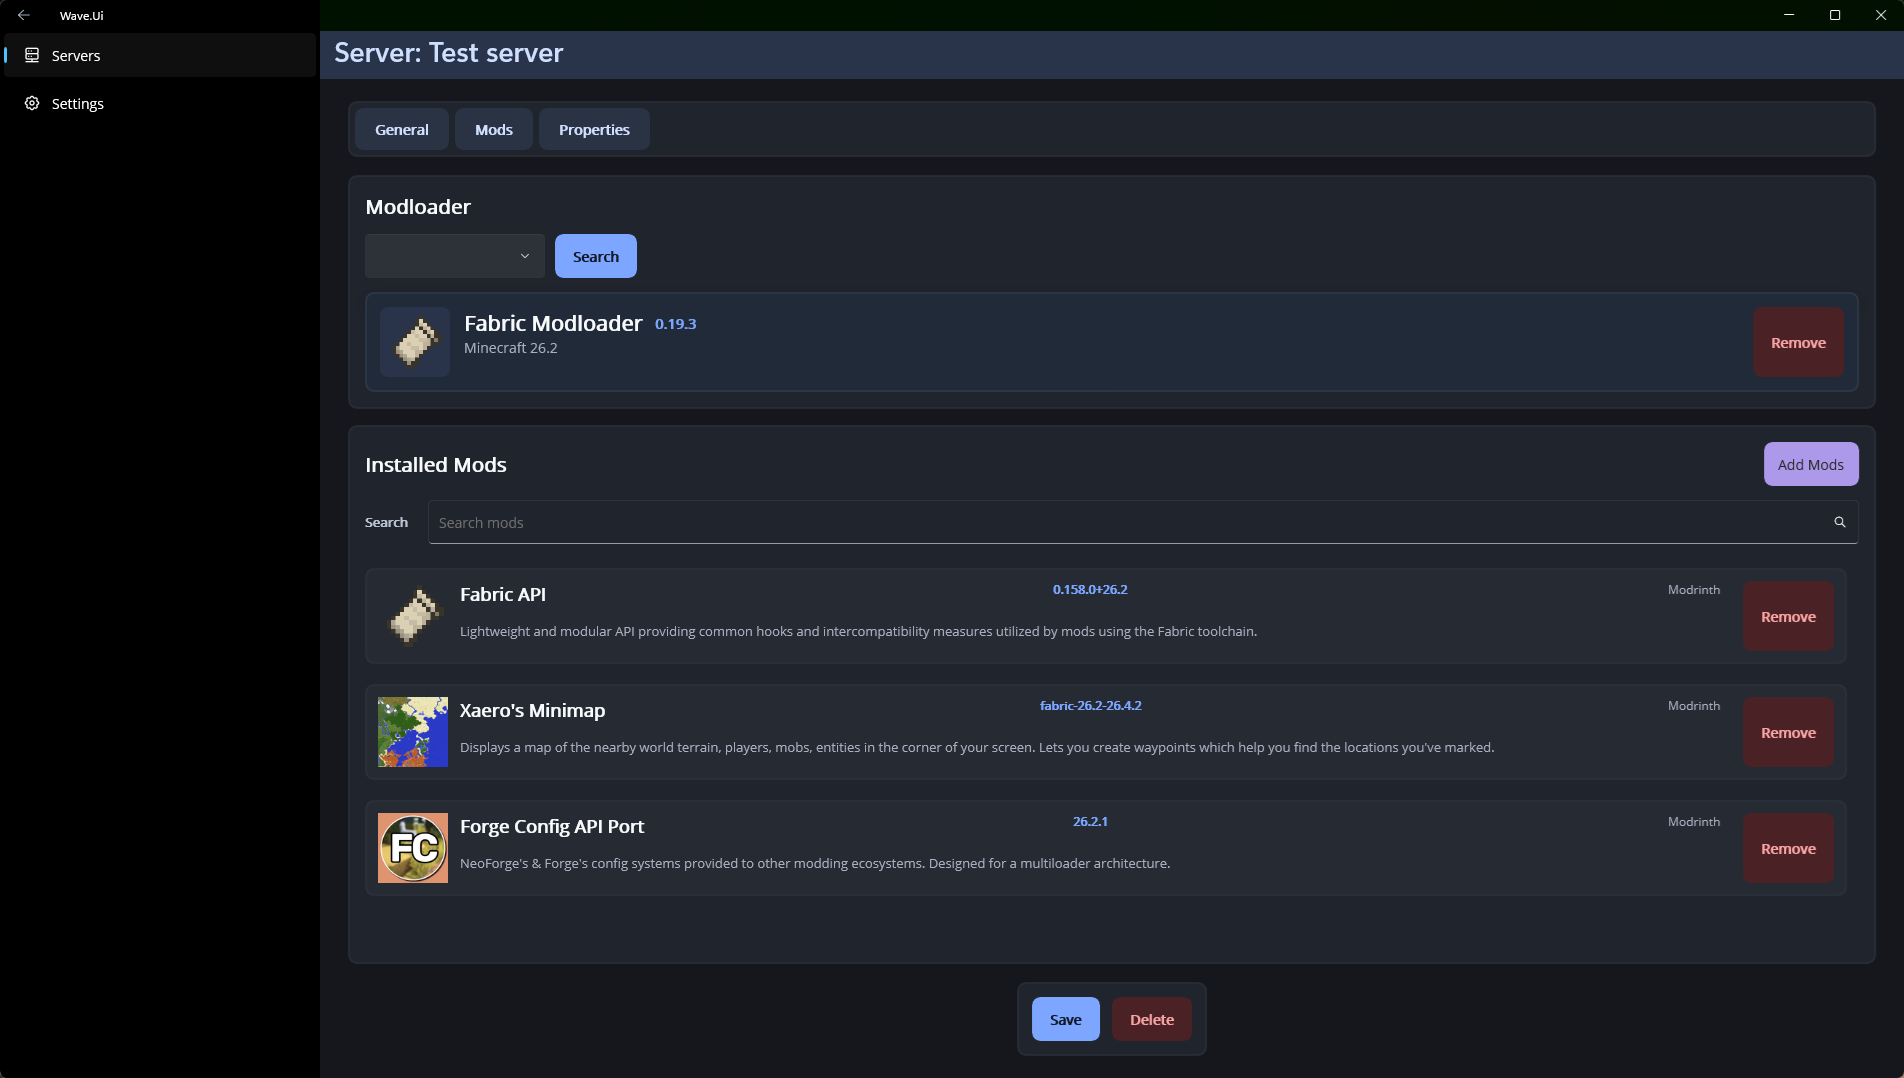
\includegraphics[width=\textwidth,height=0.72\textheight,keepaspectratio]{ServerModsPage.png}
  \caption{Installed-mods page for a server.}
  \label{fig:server-installed-mods}
\end{figure}

\subsection{Reusable forms}

The form subsystem contains text entries, check boxes, pickers and a submit button that implement a common form-element contract. Reflection helpers read and write nested model paths. This allowed the large server-properties set to be generated from definitions instead of being manually bound one property at a time.

The \texttt{Form} control discovers elements that implement \texttt{IFormElement}, assigns the current model to them and asks each element to validate itself before submission. Nested forms are deliberately skipped so that a parent form does not validate or overwrite a child form's controls. The submission method is small because traversal and validation are kept as separate responsibilities.

\begin{figure}[htbp]
  \centering
  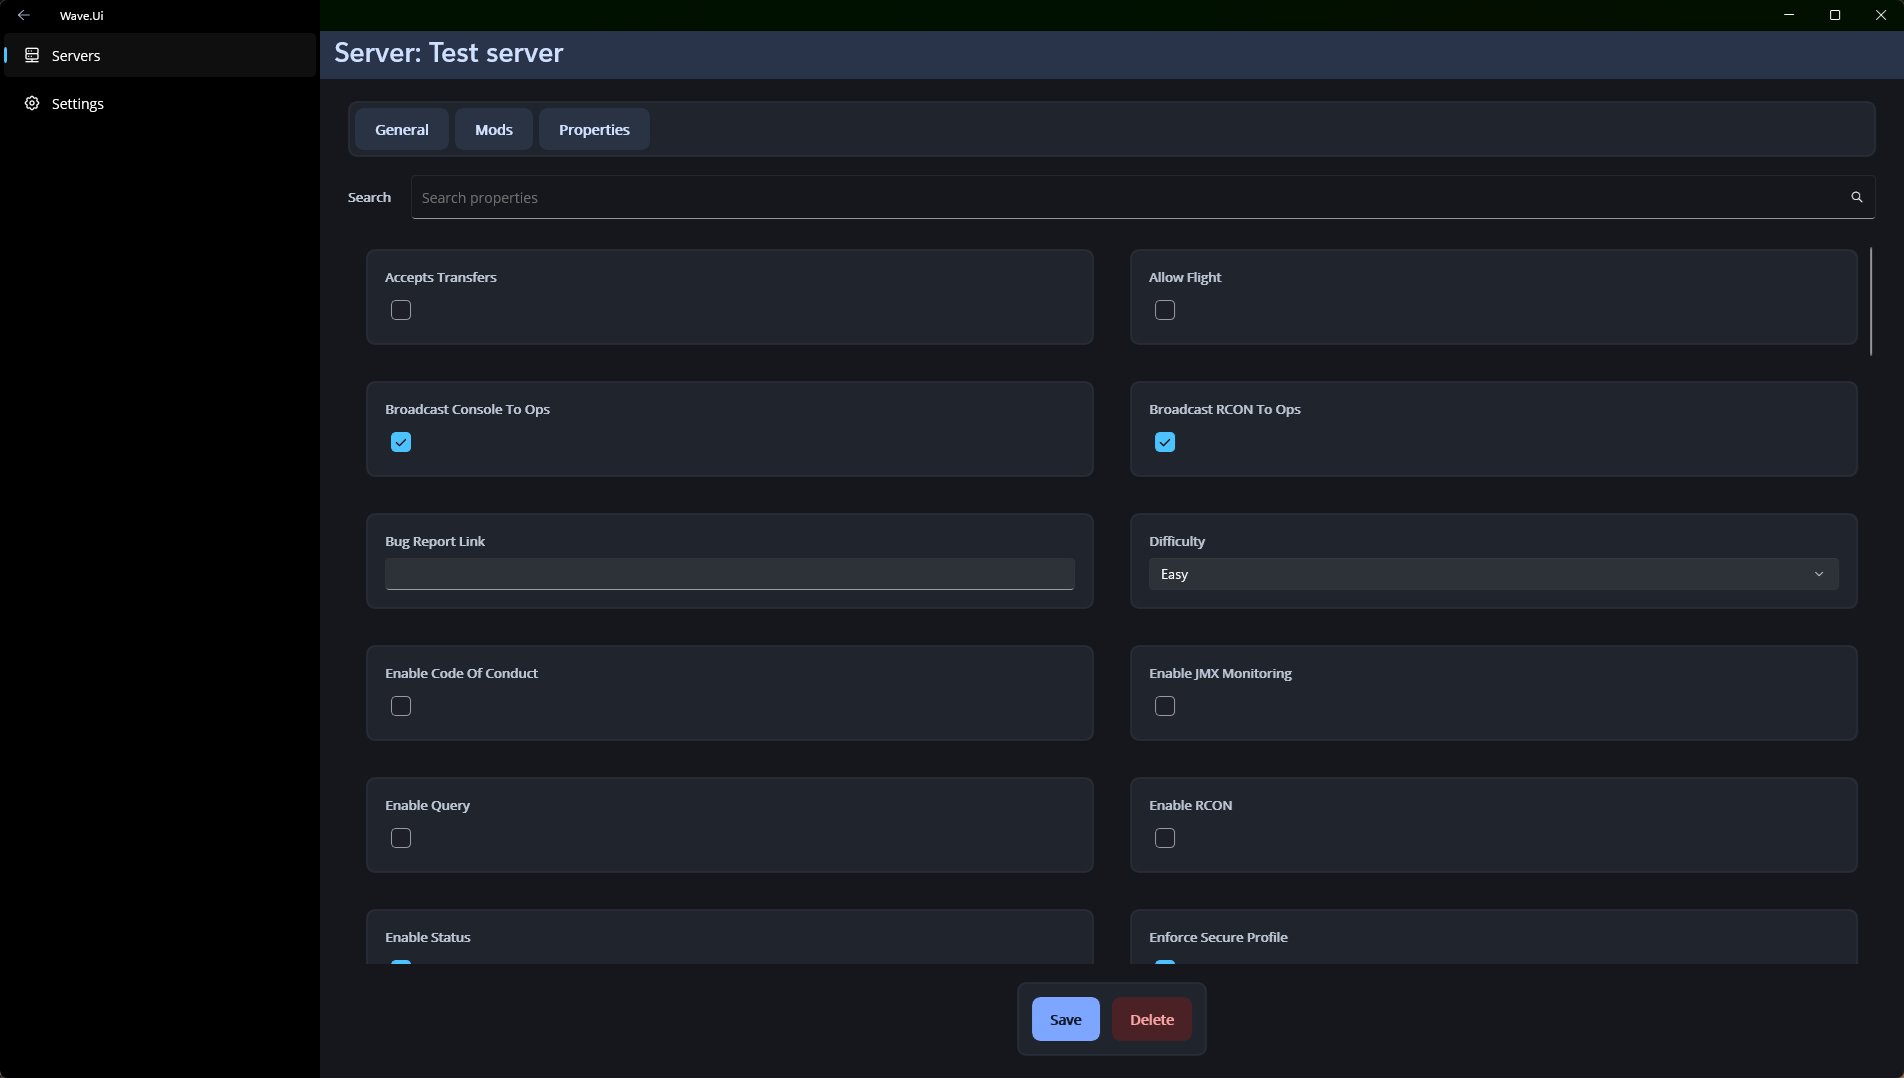
\includegraphics[width=\textwidth,height=0.72\textheight,keepaspectratio]{ServerPropertiesPage.png}
  \caption{Server-properties configuration page.}
  \label{fig:server-properties}
\end{figure}

\begin{footnotesize}
\begin{verbatim}
public void Submit()
{
    if (!Validate())
        return;

    if (SubmitCommand?.CanExecute(Model) == true)
        SubmitCommand.Execute(Model);
}
\end{verbatim}
\end{footnotesize}

Reusable forms also produced the largest schedule overrun. MAUI picker selection, generated bindings and changing binding contexts introduced cases that were not visible in simple controls. The implementation added guarded selection updates and explicit synchronization to prevent recursive changes. This work occupied the additional correction week noted in Chapter~\ref{chap:management}.

\subsection{Feedback and pagination}

Long operations set busy state and display \texttt{BusyOverlay}. The overlay communicates that the submitted action is still active and blocks accidental duplicate input. Popups present mod details and server change summaries without navigating away from the editor.

\texttt{PaginatedCollectionView} and \texttt{ObservablePaginationState} provide first, previous, next and last navigation where the supplier exposes sufficient totals. The component observes state changes and updates the displayed collection. Keeping it supplier-neutral lets Modrinth and CurseForge searches share interaction behavior despite different response schemas.

\section{Error handling}

Domain and infrastructure methods reject invalid state with specific exceptions where the caller cannot continue, such as attempting to install a second loader or execute without a Java runtime. HTTP responses are checked before files are treated as downloaded. Deserialization verifies that required response objects exist. Installer processes check their exit codes.

Expected start failures use \texttt{ServerStartResult} rather than exceptions alone. Already running, port conflict, port-mapping failure and successful start are outcomes the interface can explain. Mod installation similarly returns a structured migration result because partial compatibility is expected when providers do not publish a replacement.

The current implementation still has inconsistent edges. Some adapters write diagnostic messages to standard output or error, and several low-level failures reach the UI as general exceptions. A unified application error model and structured logging would improve diagnosis. The report does not claim that every external failure has a specialized message, only that the principal workflows distinguish the expected cases.

\chapter{Validation}\label{chap:validation}

Validation was performed against the complete application rather than against isolated adapters. The objective was to reproduce the sequence a user follows from an empty installation: obtain Java runtimes, create vanilla servers, add mod loaders and mods, migrate their configurations, execute them and finally remove all managed content. Running the same sequence on three computers also checked that the persisted paths and Windows-specific integrations did not depend on a single development machine.

The tests described in this chapter are scenario-based functional tests. They establish that the observed workflows completed in the stated environments, but they are not a performance benchmark and do not constitute proof that every provider release or network configuration is supported. Unless explicitly stated, a requirement is not considered independently validated merely because a related workflow succeeded.

\section{Environment and compatibility matrix}

The complete procedure was repeated on three computers. Two ran Windows 11, one with the Home edition and one with the Pro edition. The third ran Windows 10 Home. Hardware models and specifications were not recorded, so the environment comparison is limited to the operating-system information available.

\begin{table}[htbp]
\centering
\caption{Operating systems used for functional validation.}
\label{tab:test-environments}
\begin{tabularx}{\textwidth}{cXX}
\toprule
Device & Operating system & Executed scenario \\
\midrule
1 & Windows 11 Home & Complete end-to-end flow \\
2 & Windows 11 Pro & Complete end-to-end flow \\
3 & Windows 10 Home & Complete end-to-end flow \\
\bottomrule
\end{tabularx}
\end{table}

The same component combinations were used on every device. Java 21 was obtained from Eclipse Adoptium as a compressed package, while Java 25 was obtained from Mojang through its manifest distribution. Two server lines were exercised: Minecraft 1.21 with Forge and Java 21, and Minecraft 26.1 with Fabric and Java 25. The latter was subsequently migrated to Minecraft 26. Mods were obtained from both CurseForge and Modrinth.

\begin{table}[htbp]
\centering
\caption{Software combinations exercised during validation.}
\label{tab:compatibility-matrix}
\small
\begin{tabularx}{\textwidth}{XXXX}
\toprule
Minecraft & Selected Java & Initial loader & Additional operation \\
\midrule
1.21 & Adoptium 21 & Forge & Loader switch and mod migration \\
26.1 & Mojang 25 & Fabric & Loader switch, then downgrade to 26 \\
\bottomrule
\end{tabularx}
\end{table}

\section{Functional validation}

\subsection{Testing method}

During development, each new or modified feature was tested by running the application and exercising the corresponding workflow. The first input was a representative value, such as Minecraft 1.20 when working on version handling. Boundary or unusual values were then selected to reveal assumptions hidden by the common case. For Minecraft versions, examples included the recent 26.1 release and the old 1.0 release. This policy was exploratory rather than a fixed automated test suite, but it was applied throughout implementation and defect correction.

The final validation used a fixed twelve-step flow on each computer. It combined operations so that the output of one step became the precondition of the next. This was important for migration testing because a successful catalogue query alone does not show that installed loader and mod state can be carried into a different configuration.

\subsection{End-to-end procedure and results}

\begin{enumerate}
  \item \textbf{Java installation.} Java 21 was downloaded from Eclipse Adoptium and Java 25 from Mojang. Both installations completed successfully and appeared in the Java management interface. This exercised the compressed-package and manifest installation paths.

  \item \textbf{Automatic Java selection.} The server Java setting was changed to automatic. This allowed each server to select the installed major version required by its Minecraft release rather than assigning one runtime manually to every instance.

  \item \textbf{Server creation.} Two servers were created through the UI. One used Minecraft 26.1, which selected Java 25, and the other used Minecraft 1.21, which selected Java 21. Both server definitions and their directories were created successfully.

  \item \textbf{Mod-loader installation.} Fabric was added to the Minecraft 26.1 server and Forge to the Minecraft 1.21 server. Both loaders were installed successfully through the server editor.

  \item \textbf{Mod acquisition and dependency resolution.} Mods were downloaded from CurseForge and Modrinth. The selected set included projects with known required dependencies. In particular, Sodium Extra was installed and its required base mod, Sodium, was resolved and added correctly. This verified that a direct user selection can produce additional compatible installations through \texttt{ModManagerService}.

  \item \textbf{Mod-loader switching.} The mod loaders were switched. The application removed loader-specific mods for which the new environment was not valid, including Fabric API, while migrating mods that publish releases for both loader types, including Sodium. The resulting changes were reported to the user.

  \item \textbf{Minecraft version migration.} The Minecraft 26.1 server was downgraded to Minecraft 26. The loader and installed mods were updated to releases compatible with the target version. The server was executed successfully before and after the migration, confirming that the resulting installation remained runnable.

  \item \textbf{Property editing.} Server properties were changed through the graphical editor. The modified values were present when the servers were subsequently executed, showing that the submitted model had been written to \texttt{server.properties}.

  \item \textbf{Independent execution and commands.} Each server was started independently. Both reached successful execution with the Java runtime selected by the automatic policy. Commands were then submitted through the execution interface. The \texttt{say hello} command displayed the expected message in the in-game chat, and \texttt{gamerule keepInventory true} changed whether players retained their inventory after death. Finally, the \texttt{stop} command was submitted through the console instead of using the stop action in the UI. The Minecraft process ended normally, and Wave Launcher detected the external process termination and updated the session state accordingly.

  \item \textbf{Port-conflict handling and external access.} Start was requested while another server was already using the configured port. In both server configurations, Wave Launcher refused the second start and informed the user that the port was occupied. This confirmed the conflict check required by FR-14. During normal execution, the router also showed the server port as forwarded, and a player successfully joined from an external network. Together, these observations verified automatic port mapping and external reachability in the tested network environment.

  \item \textbf{Server deletion.} Both servers were removed through the application. The Wave Launcher servers directory was inspected afterwards and found to be empty.

  \item \textbf{Java removal.} Java 21 and Java 25 were removed after their dependent servers had been deleted. The managed Java directory was inspected afterwards and found to be empty.
\end{enumerate}

\subsection{Requirement coverage}

The scenario directly exercised viewing, creating, deleting and executing server instances; submitting commands; stopping a server from its console; adding and changing loaders; acquiring mods from both supported providers; resolving dependencies; changing Minecraft versions; managing Java installations; editing properties; detecting port conflicts; and connecting from an external network through an automatically forwarded port. The \texttt{say hello} command confirmed that commands entered in Wave Launcher reached the Minecraft server, while \texttt{gamerule keepInventory true} confirmed that a command could change the running world's rules. Submitting \texttt{stop} also showed that the launcher detected a server ending through its own console rather than through the UI. The router displayed the port mapping while the server was running, and an external player joined successfully. These observations provide direct evidence for FR-01 to FR-08, FR-10, FR-12, FR-13 and FR-14.

The flow caused loader-specific mods to be removed during migration, but it did not record a separate user-initiated removal test for FR-09 or FR-11. No pair of mods with a declared incompatibility could be found during validation, so the edge case in which the application rejects two mutually incompatible mods was not exercised. Required dependency resolution was tested successfully, but this result does not provide evidence for the incompatible-mod path.

All twelve steps completed on all three computers. In addition, no application errors were encountered during the user-evaluation sessions conducted later. The results of those sessions, including the comparison with manual server setup, are intentionally reserved for Section~\ref{sec:manual-comparison}.

\section{Comparison with manual server setup}\label{sec:manual-comparison}

Three participants with different technical backgrounds were asked to create a modded Minecraft server manually and then repeat the task with Wave Launcher. Their names are omitted, and they are identified as Subjects A, B and C. Subject A was not familiar with computers or server creation. Subject B worked in IT, understood the general purpose of a Minecraft server and reported having created servers as a child, although they no longer played the game. Subject C did not work in IT but played Minecraft regularly through the official launcher. This made Subject C familiar with the game while still fitting the project's casual-player profile, since the official launcher hides most runtime details and the participant had never created a server.

This was a small observational evaluation intended to reveal differences in the process and the obstacles encountered by each participant. The manual task was always performed first, so the Wave Launcher results may include some learning carried over from the first attempt. However, the second task still required the participants to understand a different interface and workflow.

\subsection{Test procedure}

For the manual task, participants received a short list of goals rather than detailed instructions:

\begin{enumerate}
  \item Create a server folder.
  \item Download the Minecraft server file and place it in that folder.
  \item Download Forge and install it in the server.
  \item Download mods from Modrinth.
  \item Place the downloaded mods in the server files.
  \item Configure the difficulty as \texttt{hard} and the game mode as \texttt{spectator}.
  \item Open the required router ports.
  \item Start the server and resolve any dependencies.
\end{enumerate}

No further explanation was given at the beginning. Participants could search for written or video tutorials and were also allowed to use an LLM. Assistance was provided only when a participant was severely stuck, or when an incorrect step would have prevented the remaining tasks from being completed while the participant believed it was correct. The intervention was recorded as part of the observation rather than treated as an independent completion.

Forge and Modrinth were selected to keep every participant's goal comparable. The choice was not based on an expected usability advantage, and the same broad process would have applied to Fabric and CurseForge. Specifying the provider and loader also avoided spending test time comparing ecosystems. The difficulty and game-mode values were chosen so that each participant had to locate and edit values inside the long \texttt{server.properties} file rather than leaving the defaults unchanged.

The Wave Launcher task expressed the same intended result in four user-level steps:

\begin{enumerate}
  \item Create a server with difficulty set to \texttt{hard} and game mode set to \texttt{spectator}.
  \item Add Forge.
  \item Add mods.
  \item Start the server.
\end{enumerate}

The difference in the number and type of steps already illustrates part of the abstraction provided by the application. The manual list exposes file placement, loader installation, configuration-file editing, router setup and dependency resolution as separate responsibilities. The Wave Launcher list describes the result the player wants, while the application carries out most of those technical operations internally.

All timestamps were measured from the beginning of the corresponding task and have been standardized as minutes and seconds in Table~\ref{tab:manual-wave-users}. The reduction column compares each participant's Wave Launcher time with their manual time.

\begin{table}[htbp]
\centering
\caption{Completion times for manual setup and Wave Launcher.}
\label{tab:manual-wave-users}
\small
\begin{tabularx}{\textwidth}{cXrrr}
\toprule
Subject & Background & Manual & Wave Launcher & Time reduction \\
\midrule
A & Limited computer experience; no server experience & 18:39 & 05:00 & 73.2\% \\
B & IT background; previous server experience & 22:14 & 02:08 & 90.4\% \\
C & Regular Minecraft player; no server experience & 18:23 & 04:05 & 77.8\% \\
\midrule
Mean & & 19:45 & 03:44 & 81.1\% \\
\bottomrule
\end{tabularx}
\end{table}

\subsection{Manual creation across participant backgrounds}

Subject A completed the folder and vanilla-server download but initially executed the JAR from the Downloads directory. Minecraft generated its files there, after which the participant moved some files into the intended server folder without moving the executable itself. Command-line directory navigation caused further difficulty, although the participant found and edited \texttt{eula.txt} without assistance. By 05:00, the vanilla files had been moved into the server folder.

The Forge stage exposed version and directory problems. Subject A downloaded the latest Forge installer without first comparing it with the selected Minecraft version, consulted two tutorials and created an unnecessary nested Forge directory. The participant then attempted to run the server from that directory. While browsing Modrinth, they first selected ETF for Fabric, noticed the loader mismatch, and replaced it with a compatible TerraBlender release. Assistance was needed to explain that the mod belonged in a \texttt{mods} directory. The participant later found and correctly changed the difficulty and game-mode entries, but needed to be told to enter \texttt{stop} before restarting the server. Port forwarding was unfamiliar and required direct explanation. The final Forge server was running at 18:39.

Subject B approached downloads more cautiously because of their IT background. They checked whether \texttt{minecraft.net} was a legitimate source and scanned the Forge JAR with VirusTotal. They also compared the Forge and Minecraft versions before installation. Even with this background, uncertainty remained about the required order: the participant questioned whether the vanilla server should be run before Forge and initially started searching for mods before installing the loader.

Compatibility selection took a noticeable part of Subject B's test. Create (the first selected mod) was unavailable for Minecraft 26.2, Sodium did not provide a Forge release for the chosen combination, and the participant eventually selected Xaero's Minimap. They searched for instructions, installed Forge at 12:33 and, like Subject A, created an unnecessary nested folder. The mod was placed in that nested installation. The configuration properties were changed correctly after an online search. Router configuration then required searches for the gateway, local IP address, protocol, Minecraft port and forwarding settings. Assistance was needed to identify the port-forwarding page and to clarify that the internal and external ports should match. At the end, the participant read the process output but needed to be told that Minecraft's \texttt{Done} line indicates successful startup. Completion was recorded at 22:14.

Subject C moved through the early download steps quickly. They created the folder, downloaded the vanilla server by 00:40, compared Forge versions and obtained the recommended installer by 01:11. They then searched for instructions on installing a loader and used the batch command provided on the Minecraft download page to start the vanilla server. EULA acceptance was completed at 04:14. Assistance was needed at 06:30 to explain that the Forge installer itself had to be executed. After that clarification, the participant selected the server-install option and chose the correct directory.

Subject C filtered Modrinth by Minecraft version, downloaded Xaero's Minimap and needed clarification that it belonged in a \texttt{mods} subdirectory. They correctly changed both requested properties by 11:00. Port forwarding was again the largest unfamiliar area. The participant found the default gateway with \texttt{ipconfig}, but required an explanation of the router interface and the port to open. When starting the completed server, they first launched the vanilla JAR, which excluded Forge and its mods. They were then directed to the Forge-generated batch file. At 18:23, they still could not determine from the log whether startup had succeeded and needed to be shown the \texttt{Done} line.

The three manual attempts show both differences and similarities between skill levels. Subject A had the most difficulty with directory organization and command-line navigation. Subject B performed more security and compatibility checks and understood more of the terminology, but this did not produce the shortest completion time. In fact, the additional verification and online research made Subject B's manual attempt the longest. Subject C was faster in the first download stages because of familiarity with Minecraft, but that familiarity did not extend to loader execution, mod directories, networking or server logs.

The manual completion times require an important qualification. Subject B's basic understanding of servers allowed them to attempt the port-forwarding process rather than stopping immediately. They independently searched for the router gateway, local IP address, required protocol and Minecraft port before receiving limited clarification about the router settings. Subjects A and C reached an impasse at this stage and did not know how to continue, so they were directly told how to configure the forwarding rule. This assistance allowed their tests to proceed sooner. Subject B's longer manual time therefore does not indicate poorer performance than Subjects A and C. Part of the difference comes from spending more time attempting the most technical step independently, while the other two participants received the procedure after becoming stuck. For this reason, the recorded times describe the observed sessions but should not be used alone to rank the participants' manual ability.

All three participants eventually encountered uncertainty about the relationship between the vanilla server, Forge and the selected mods. Subjects A and C needed help identifying the mod directory, while Subject B searched for instructions and initially proceeded before the loader was installed. Subjects A and B created unnecessary nested Forge directories, and Subject C first executed the vanilla server instead of the Forge launch script. One possible reason for the nested directories is the Forge installer's warning when the selected destination already contains files. The warning is displayed in red text, which can reasonably be interpreted as an error even though selecting the existing server directory is normal and required. Creating a new empty subdirectory may therefore appear to the user as the safer option. The observations do not establish that this warning was the sole cause, but the same behavior in two participants suggests that the installer feedback may contribute to the confusion. Overall, these results indicate that general computer knowledge and familiarity with Minecraft help with individual actions, but neither one alone gives a clear mental model of the complete modded-server installation.

\subsection{Wave Launcher use across participant backgrounds}

With Wave Launcher, Subject A created the server, selected a version, accepted the EULA and configured the requested difficulty and game mode. They asked about the message of the day, execution flags and Java selection, which indicates that some labels still assume technical knowledge. After creation, the participant correctly returned to the editor and selected Forge. They first used the installed-mod filter instead of the add-mod button, but after being shown the correct button they added TerraBlender through CurseForge and started the server. The complete task took 05:00.

Subject B selected Minecraft 1.21.1, the requested game mode and difficulty, accepted the EULA and manually chose an existing Java installation, although automatic selection was sufficient. The participant added Forge by 01:00. They were unsure which Forge release to select and were advised to choose the latest compatible option. In the mod popup, they initially searched without selecting a supplier. Once this requirement was explained, they found and added Hydraulic Machines, saved the server and started it at 02:08.

Subject C created and configured the server, then paused at 00:54 to search online for the meaning of execution flags. They opened the existing server at 01:30, selected Forge 65.1.2 and, like Subject A, first tried the installed-mod search field rather than the add-mod button. After being redirected to the popup, they selected Modrinth, found a Xaero's Minimap, selected a version and added it by 03:43. The changes were saved at 04:02 and the server was running at 04:05.

Background had less effect on completion with Wave Launcher than it did on the path taken during manual creation. Subject B was the fastest, which is consistent with greater familiarity with software configuration, but Subjects A and C also completed the workflow in five minutes or less. The difficulties were mostly local interface-discovery issues rather than server-administration problems. Subjects A and C confused the installed-mod filter with the add-mod control. Subject B attempted a search before choosing a supplier. Subjects A and C questioned execution flags, and Subject A also needed clarification about Java selection and the message of the day.

These observations reveal useful areas for UI improvement. The add-mod action could be made more prominent, and the supplier requirement could be explained before a search is attempted. Optional technical fields such as execution flags could include short descriptions or remain collapsed for casual users. Java's automatic-selection behavior should also be clearer so that users do not assume they must understand or select a runtime manually. None of these issues prevented completion once the relevant control was identified.

\subsection{Manual setup compared with Wave Launcher}

Wave Launcher reduced the mean completion time from 19:45 to 03:44, an observed reduction of 81.1\%. The individual reductions ranged from 73.2\% to 90.4\%. With only three participants and a fixed task order, these values should be read as results of this evaluation rather than as estimates for the wider population. Even so, the time difference is supported by a visible reduction in both the number of operations and the amount of external research.

Some activities were common to both methods. Participants still had to choose a Minecraft version, a loader and a mod, approve the EULA, configure the requested gameplay properties and start the server. Compatibility concepts also remained visible to some extent, since users selected Forge and a provider. The difference was where responsibility for the consequences of those choices was placed. During manual creation, participants had to obtain the correct artifacts, decide where they belonged, use the correct launch file and interpret provider and server output. In Wave Launcher, these actions were coordinated behind the selected options.

The largest manual difficulties were network configuration and determining whether the server had started correctly. Every participant needed help with port forwarding or with specific router values. Two participants could not independently recognize successful startup in the logs, and the remaining participant also needed guidance to search for the \texttt{Done} message. Mod and loader compatibility created a related problem: participants selected unavailable or incompatible combinations, installed files in the wrong order, or launched the vanilla server without the loader. A manual failure at any of these points left the participant to determine whether the problem came from Minecraft, Java, Forge, a mod, a missing dependency, the directory layout or the network.

Wave Launcher directly addresses these two main obstacles. It requests and releases the router mapping when the server session starts and stops, checks for a local port conflict, and reports mapping failure as a startup result. The validation described earlier also confirmed a visible router mapping and a successful connection from an external network. For execution, the application starts the correct vanilla or loader JAR with the selected Java runtime and tracks the resulting process, so the UI can represent whether a session is running. Loader and mod searches are filtered by the selected Minecraft environment, required dependencies are resolved automatically, and migration results report components that cannot be retained. The application therefore does more than shorten the manual instructions. It takes responsibility for the two areas that caused the most uncertainty in all three observations: network exposure and the combined interpretation of startup, loader, mod and dependency state.

\section{Known defects and limitations observed during testing}

No known reproducible defects remain at the time of writing. Errors found during development and exploratory testing were corrected before the final three-device procedure. This statement describes the current observed state rather than claiming that the program is defect-free. The test matrix is finite, provider data can change, and hardware or network configurations outside the three computers may reveal additional failures.

Java installation is limited to compressed packages, such as ZIP and TAR.GZ archives, and manifest-based distributions. Eclipse Adoptium also publishes MSI installers, but that installation path was excluded after it introduced disproportionate complexity during development. Wave Launcher therefore obtains Adoptium runtimes through portable compressed packages and Mojang runtimes through manifests. This avoids system-wide installer behavior but means that a provider release available only as an MSI cannot be installed by the current adapters.

Loader support is limited to Forge and Fabric. Other active ecosystems, including NeoForge and Quilt, were not implemented. They are more commonly selected by experienced or power users, whereas Wave Launcher is scoped around the needs of casual players. The port and adapter design allows another loader catalogue and installer to be added later.

Finally, successful execution on Windows 10 Home, Windows 11 Home and Windows 11 Pro does not establish support for other operating systems. The interface uses .NET MAUI, but process execution, device information and the validated network behavior remain Windows-specific in the current release.
